\chapter{Introduction, Background \& Objectives}

%This section should discuss your preparation for the project, including background reading, your analysis of the problem and the process or method you have followed to help structure your work.  It is likely that you will reuse part of your outline project specification, but at this point in the project you should have more to talk about. 

%\textbf{Note}: 

%\begin{itemize}
  % \item All of the sections and text in this example are for illustration purposes. The main Chapters are a good starting point, but the content and actual sections that you include are likely to be different.
   
   %\item Look at the document on the Structure of the Final Report for additional guidance. 
   
%\end {itemize}

%Outline:
%What problem was tackled?
%Why was that problem tackled?
%How (in outline) was the problem tackled?
%Clear statement of project aim and objectives
%Guide to subsequent chapters
%Usually drafted early, and finished last

\section{Introduction}
%\section{Background}
%What was your background preparation for the project? What similar systems did you assess? What was your motivation and interest in this project?
Route planning has been a useful tool for thousands of years; even before we started drawing maps, and routes were planned relative to landmarks and star-constellations. In our modern society, route-planning systems are becoming increasingly more accurate and commonplace in our daily lives. These systems can be used by anyone: From tourists trying to find the nearest public toilet, to the Mars rovers\cite{marsRover} - boldly going where no one has gone before.

A significant amount of money and effort has been put into extensively mapping our world \cite{OSM,gmaps1,gmaps2,geofabrik}, which in turn has provided route-planning systems even more data to work with -- making them more accurate and useful than ever before.

Route-planning systems are of course only practical to use if they are able to plan routes that their users are able to follow, which is unfortunately often not the case for persons with reduced mobility (PRM). Most public route-planning systems focus on providing routing-services to very large, generalised groups of people - like pedestrians, cyclists or motorists, but very rarely consider PRMs as a separate group to these.

PRMs are often categorised as pedestrians, and are therefore given routes intended for people who are able to walk up stairs, cross streets with elevated curbs, climb steep inclines, etc. Many PRMs are able to pass these obstacles with some assistance from someone else, but this does not apply to everyone; their wheelchair might be too heavy to lift manually, they might be old and/or have a form of muscular atrophy that makes it hard for them to keep their balance, or there might not be anyone around able to give them the help they need.

PRMs could try following routes intended for cyclists, as these usually avoid stairs, but they might still contain tall curbs, steep slopes, etc. Bike-routes also tend to be noticeably longer than pedestrian routes, so these may not always be suitable for many PRMs either.

As built-up areas are often particularly challenging environments to navigate for PRMs, the project developed as part of this dissertation has focused most of its attention to areas like this. Additionally: Because Aberystwyth University has made a notable effort to make its campuses more accessible for everyone in recent years, and because there are more people with disabilities in higher education now than ever before\cite{tinklin2004}, this project has put its main focus on the Aberystwyth University campuses.

This project builds upon the author's Major project for their BSc degree at Aberystwyth University (\textquotedblleft Access Aber - Pathfinding\textquotedblright), completed in 2015, which in turn was inspired by a separate system developed by Aberystwyth University in the summer of 2014: \textquotedblleft Access Aber\textquotedblright.

\begin{figure}
	\centering
	
	
	\subfigure[Route for Persons with Reduced Mobility]{\frame{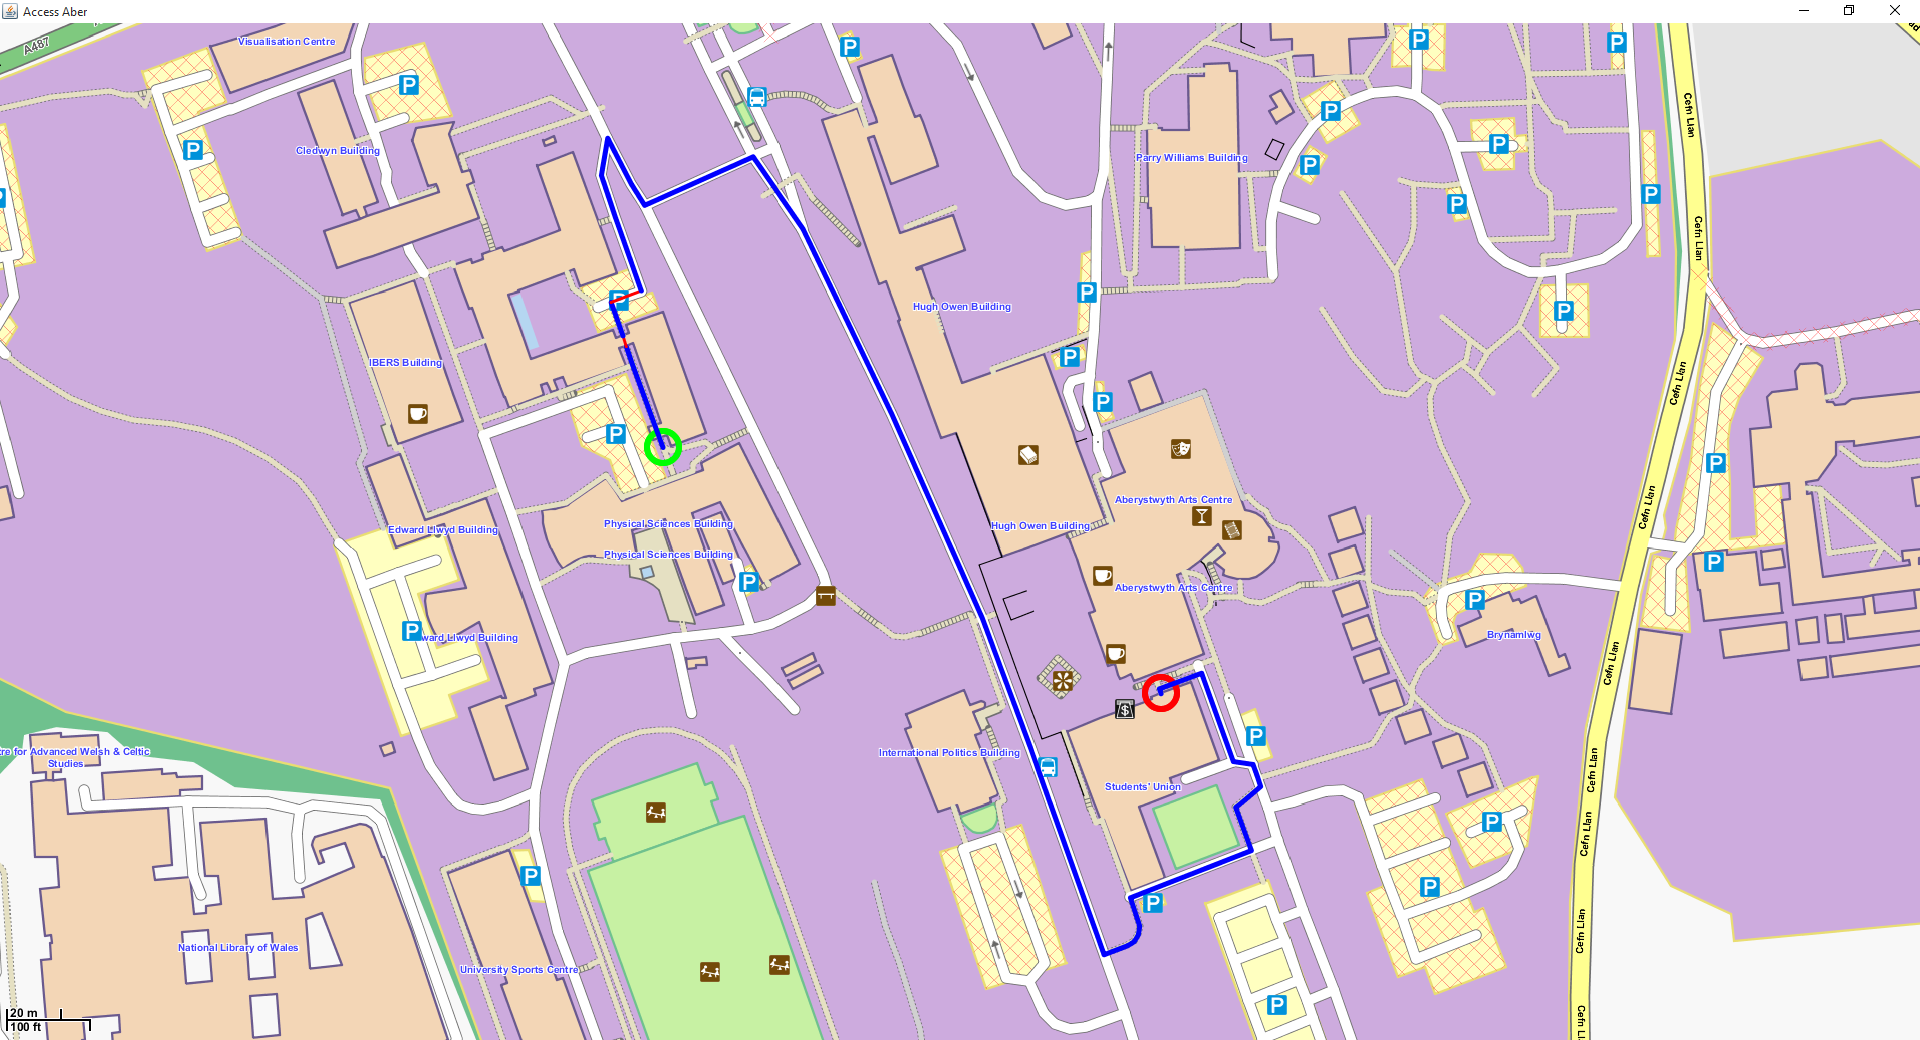
\includegraphics[keepaspectratio, width=\columnwidth]{Images/AStar_CSdept-SU}}}
	
	\subfigure[Route for able-bodied pedestrians]{\frame{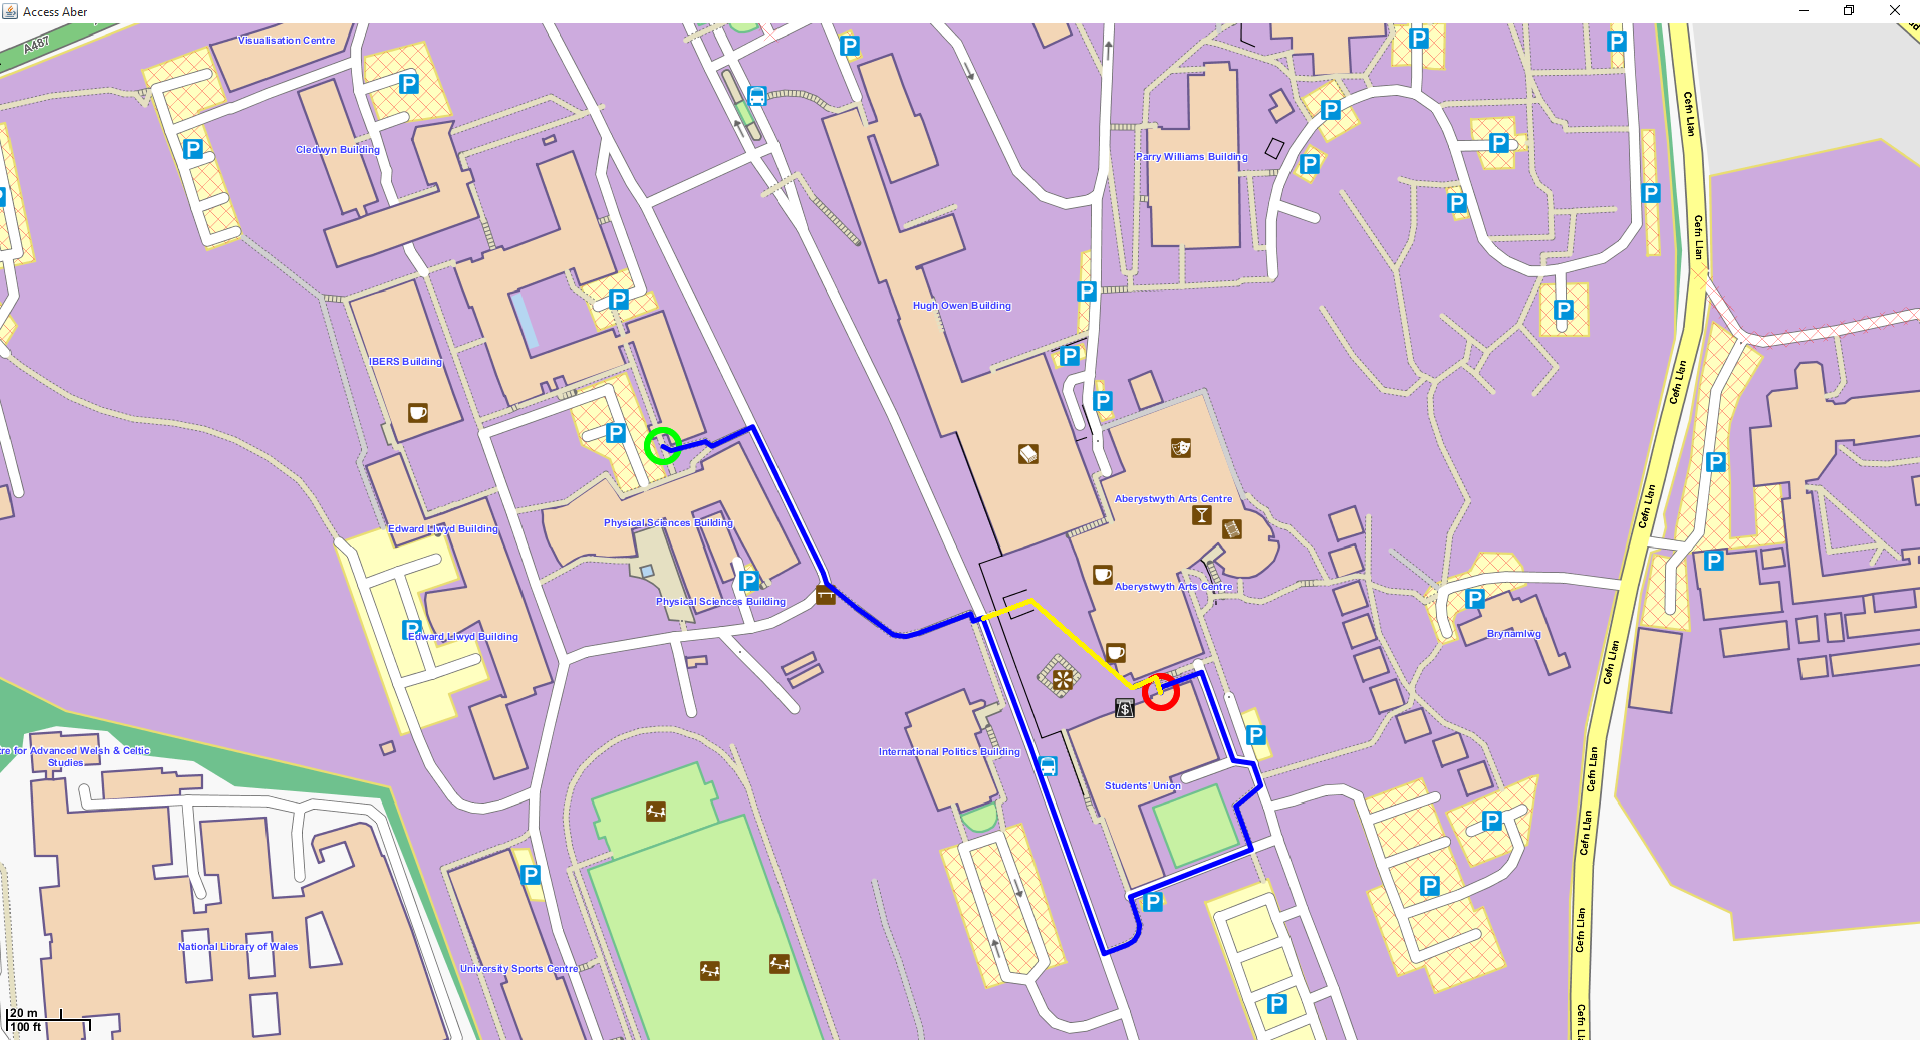
\includegraphics[keepaspectratio, width=\columnwidth]{Images/AStar_CSdept-SU_Foot}}}
	\caption[Longer routes for Persons with Reduced Mobility]{These images show two different routes from the computer-science department (\textit{IMPACS}) on Penglais campus, to the Students' Union. As there are many stairs in the way, many PRMs are forced to follow a far longer route than an able-bodied person would. The yellow line in (b) (hand-drawn by me -- starting where (a) and (b) intersect) shows the actual path an able-bodied pedestrian would take. The route in (b) is likely sub-optimal because data is missing from OpenStreetMap's database; Mapzen on \url{openstreetmap.org} finds the same route as (b) (29.September.2016).}
	\label{fig:longerRoutePRM}
\end{figure}

\section{Analysis}
%Taking into account the problem and what you learned from the background work, what was your analysis of the problem? How did your analysis help to decompose the problem into the main tasks that you would undertake? Were there alternative approaches? Why did you choose one approach compared to the alternatives? 

%There should be a clear statement of the objectives of the work, which you will evaluate at the end of the work. 

%In most cases, the agreed objectives or requirements will be the result of a compromise between what would ideally have been produced and what was felt to be possible in the time available. A discussion of the process of arriving at the final list is usually appropriate.
The goal of this project is to show that it is possible to plan accessible routes for PRMs, but more importantly: The project needs to show why more route-planning systems should consider PRMs to a much larger degree than they currently do, and that some areas on the Aberystwyth University campuses could still be made more accessible than they currently are.

The system developed as part of this dissertation has to identify the most important aspects of route planning, and replicate this in a route-planning system made specifically for PRMs.
These aspects include, but are not limited to: calculating routes in near-real-time, having a low memory-footprint, employing optimal and complete routing-algorithms, and of course finding appropriate routes for the target users.

The process of extensive and accurate mapping of Nodes (or individual points of navigational data) is a task beyond the scope of this project, so this data will have to be retrieved from a third party. This will be discussed in more detail later in this report.

The A Star (A*) search-algorithm has been chosen as the default algorithm for route-planning (The reasoning behind this will be explained later), but three other search-algorithms have also been implemented -- each of which can be selected by providing the system with a specific command when it is started; See the \textit{README.txt} packaged together with the source-code. 

Most commercial route-planners use search-algorithms able to abstract routing-data into large blocks connected to each other by only a few roads, which lets them plan incredibly long routes seemingly instantly by jumping directly from block to block, rather than looking at the road-networks inside in detail. This abstraction often leads to a loss of accuracy however, as the algorithms tend to favour main roads over side roads which may provide a slightly more time/fuel efficient route. For most people, this slight increase in path-costs do not matter too much in their day-to-day lives, but as explained later in this document, PRMs often need to follow significantly longer routes than able-bodies pedestrians, due to their physical limitations making it hard to pass certain obstacles. Because of this, the routes returned to PRMs by a route-planning system should always be as optimal as possible to avoid any further inconvenience. This does not mean that the routing-data cannot be abstracted at all however -- and you will see later -- so it is still possible to take certain measures to reduce runtimes and memory-requirements.

\newpage
\section{Process}
%You need to describe briefly the life cycle model or research method that you used. You do not need to write about all of the different process models that you are aware of. Focus on the process model that you have used. It is possible that you needed to adapt an existing process model to suit your project; clearly identify what you used and how you adapted it for your needs.
The life cycle models used for this project are Test Driven Development (More on this later), and the Spiral Model.

The Spiral Model makes it easier to select specific parts of the system to develop within a certain time-frame, and to develop these parts properly, as it encourages more detailed planning. The following are the four main steps in the Spiral Model:
\begin{enumerate}
	\item Determine objectives
	\subitem Clearly specify what functionality we expect to be present at the end of this iteration.
	\item Identify and resolve risks
	\subitem Find the best solution(s) for solving the problem at hand, but which will still allow us to finish within the planned time-frame
	\subsubitem This might mean sacrificing a good solution for a slightly worse one if we expect that the best solution would take too long to implement -- ie. lowering the risk of not being able to finish the project on time.
	\item Development and Test
	\subitem Implement the solution(s) found in the previous step, and test whether they break any new or existing functionality.
	\item Plan the next iteration
	\subitem Determine which part of the system needs the most attention, and make plans relative to that.
\end{enumerate}

Extreme programming (XP) was also considered for this project, but was decided against because the author knew from experience that they needed a slightly more plan-driven approach to development to make sure that the system was finished on time. The Spiral Model makes it easier to focus on one aspect of the system at a time, and makes sure that that aspect is implemented properly. It does this by having a step dedicated to finding and evaluating alternative approaches based on the risk involved in implementing them. This risk could be: time vs memory requirements, expected difficulty of coding, etc.

After one iteration of the spiral is complete, we are able to move on to another part of the system. This makes it much easier to stop optimising every aspect of the system, and instead prioritise creating a finished product.

Testing has been a crucial part of development, and every method in the source-code has one or more tests associated with it, but again: This will be discussed in more detail later. 